\chapter{Pruebas}

Según la metodología ``cascada'', la fase de implementación se cierra cuando se realizan las pruebas respectivas sobre los módulos implementados. Para probar en su totalidad el sistema de video-vigilancia se realizaron pruebas en el móodulo de cámara y el servidor.\\

\section{Prueba de conexión de cámaras}
En la tabla \ref{con_modulo_cameras} se detalla la prueba realizada sobre la conexión de una nueva cámara en el módulo de cámaras.

\begin{table}[H]
    \caption{Detalle de prueba de conexión}
    \label{con_modulo_cameras}
    \begin{center}
        \begin{tabular}{|>{\centering}p{0.3\textwidth}|m{0.6\textwidth}<{\centering}|} 
            \hline
            \textbf{Título de la prueba} & \textbf{Única cámara conectada} \\
            \hline
            \textbf{Descripción} & El servidor se encuentra en ejecución y una instancia del módulo de cámaras se conecta al servidor. No existen más cámaras conectadas.\\
            \hline
            \textbf{Comportamiento obtenido} & 
            \begin{itemize}
                \item El servidor registra la desconexión y lo muestra en consola.
                \item El servidor notifica al usuario por medio de correo electrónico.
                \item El servidor notifica al usuario por medio de whatsapp.
                \item La notificación provee información sobre la fecha y hora de la desconexión.
                \item La notificación detalla que no hay más conexiones.
            \end{itemize} \\ 
            \hline
            \textbf{Estado de prueba} & Exitoso \\
            \hline
        \end{tabular}
        \begin{center}
            Fuente: Elaboración propia.
        \end{center}
    \end{center}
\end{table}

El servidor se encuentra a la espera de nuevas conexiones y en la figura \ref{camera_connected_one_camera} se visualiza los mensajes mostrados en su interfaz a partir del comportamiento esperado del módulo.\\

\begin{figure}[H]
    \begin{center}
        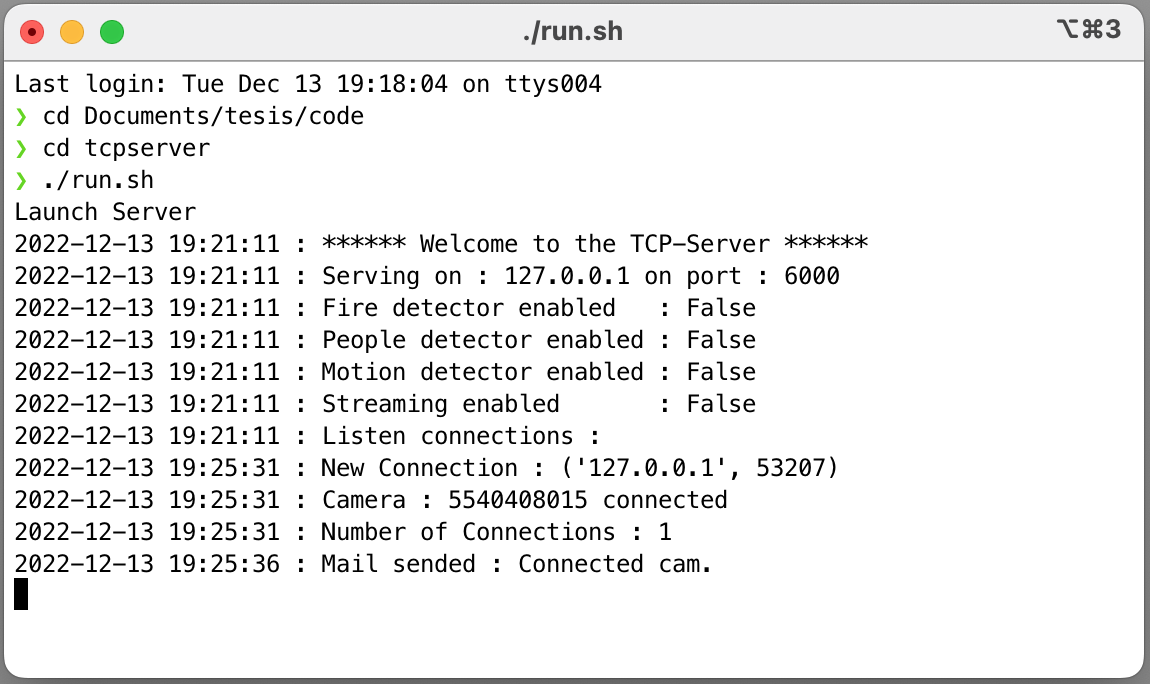
\includegraphics[width=13cm]{img/capitulo_6/server_cam_connected.png}
    \end{center}
    \begin{center}
        \caption{Mensajes de la interfaz del servidor.}
        Fuente : Elaboración propia
        \label{camera_connected_one_camera}
    \end{center}
\end{figure}

En la figura \ref{mail_one_camera_connected} se visualiza el correo electrónico que el usuario recibe como notificación después de la conexión de una cámara en el sistema.\\

\begin{figure}[H]
    \begin{center}
        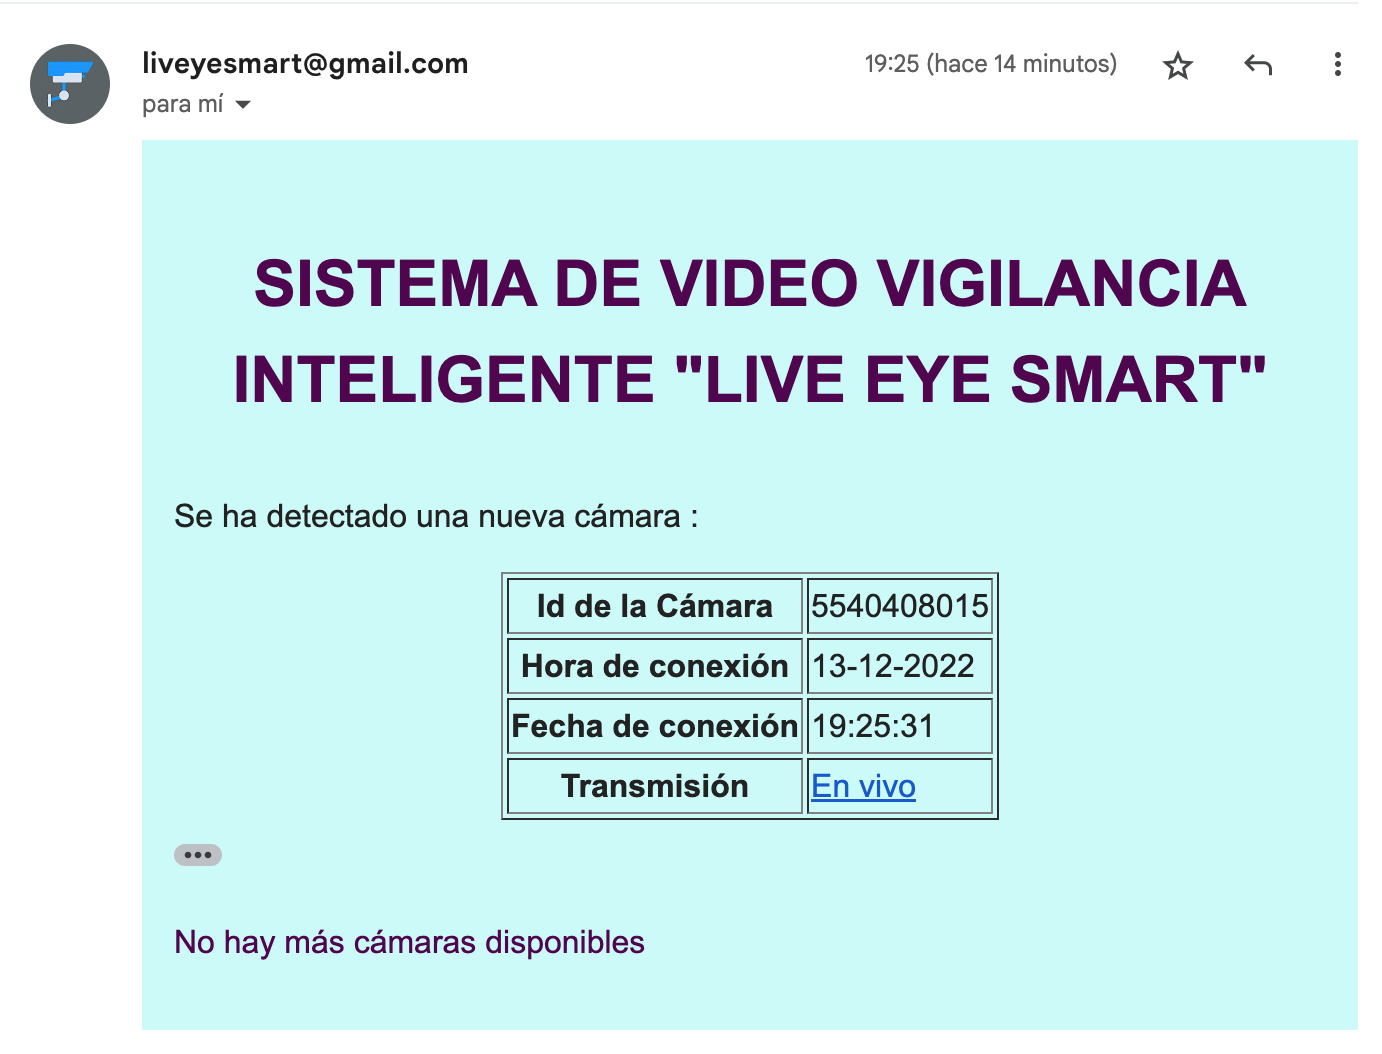
\includegraphics[width=11cm]{img/capitulo_6/mail1.png}
    \end{center}
    \begin{center}
        \caption{Notificación por correo - Una cámara conectada.}
        Fuente : Elaboración propia
        \label{mail_one_camera_connected}
    \end{center}
\end{figure}

En la tabla \ref{many_cameras_connected_table} se detalla la prueba realizada en el caso de cuando se tiene varias cámaras conectadas y se conecta una cámara adicional.\\

\begin{table}[H]
    \caption{Conexión de varias cámaras}
    \begin{center}
        \begin{tabular}{|>{\centering}p{0.3\textwidth}|m{0.6\textwidth}<{\centering}|} 
            \hline
            \textbf{Título de la prueba} & \textbf{ Más de una cámara conectada} \\
            \hline
            \textbf{Descripción} & El servidor se encuentra en ejecución y una instancia del módulo de cámaras se conecta al servidor. Existen más de una cámara conectada.\\
            \hline
            \textbf{Comportamiento obtenido} & 
            \begin{itemize}
                \item El servidor acepta la conexión y lo muestra en consola.
                \item El servidor notifica al usuario por medio de correo electronico.
                \item La notificación provee información sobre la fecha y hora de la conexión, compartiendo el enlace para la transmisión en vivo.
                \item La notificación provee la misma información de las demás cámaras conectadas al servidor.
            \end{itemize} \\ 
            \hline
            \textbf{Estado de prueba} & Exitoso \\
            \hline
        \end{tabular}
        \label{many_cameras_connected_table}
        \begin{center}
            Fuente: Elaboración propia.
        \end{center}
    \end{center}
\end{table}

En la figura \ref{n_cameras_connected}, se visualiza los mensajes que se muestran en la consola del servidor cuando se conecta una cámara adicional.

\begin{figure}[H]
    \begin{center}
        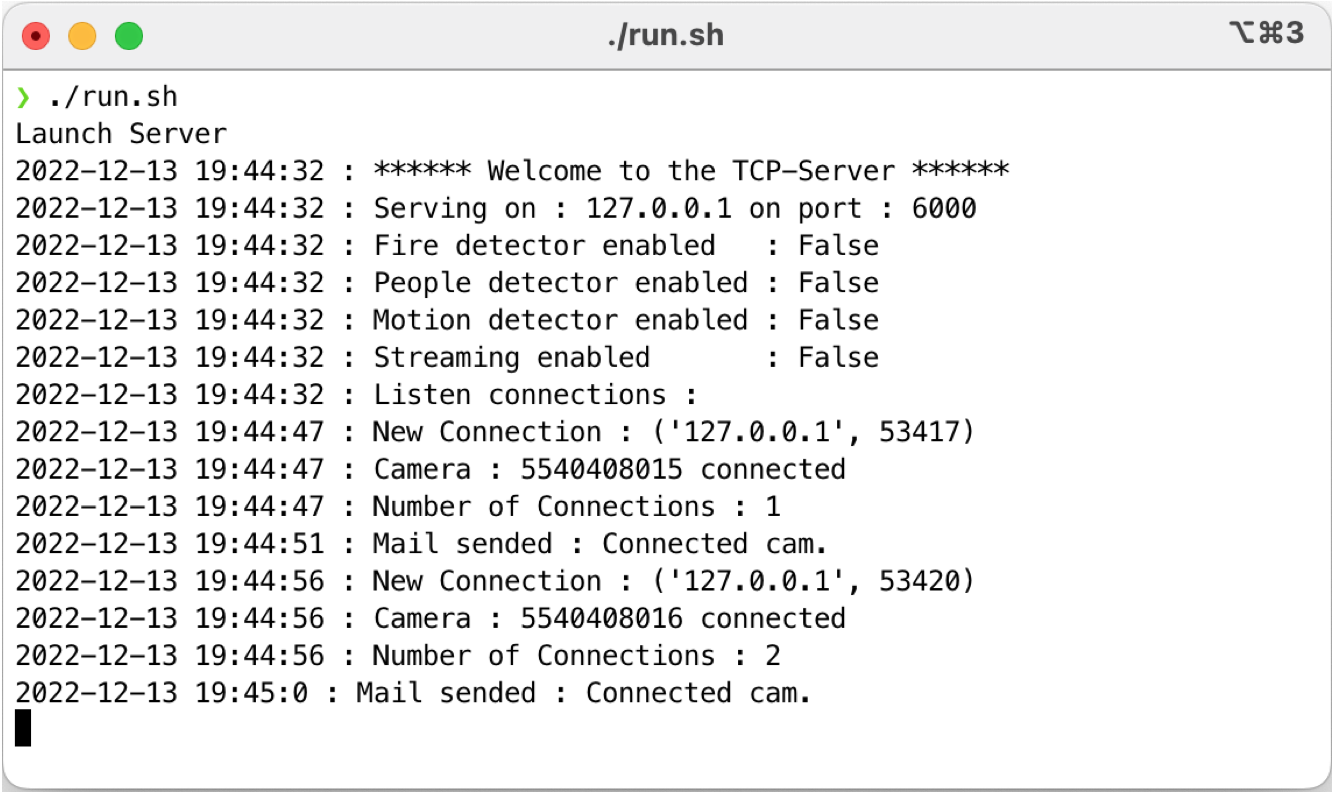
\includegraphics[width=11cm]{img/capitulo_6/server_cam_connected_more_cams.png}
    \end{center}
    \begin{center}
        \caption{Interfaz de servidor en más de una cámara conectada.}
        Fuente : Elaboración propia
        \label{n_cameras_connected}
    \end{center}
\end{figure}

En la figura \ref{notif_mail_n_cameras} se visualiza la notificación por correo electronico recibido cuando se conecta una cámara adicional.

\begin{figure}[H]
    \begin{center}
        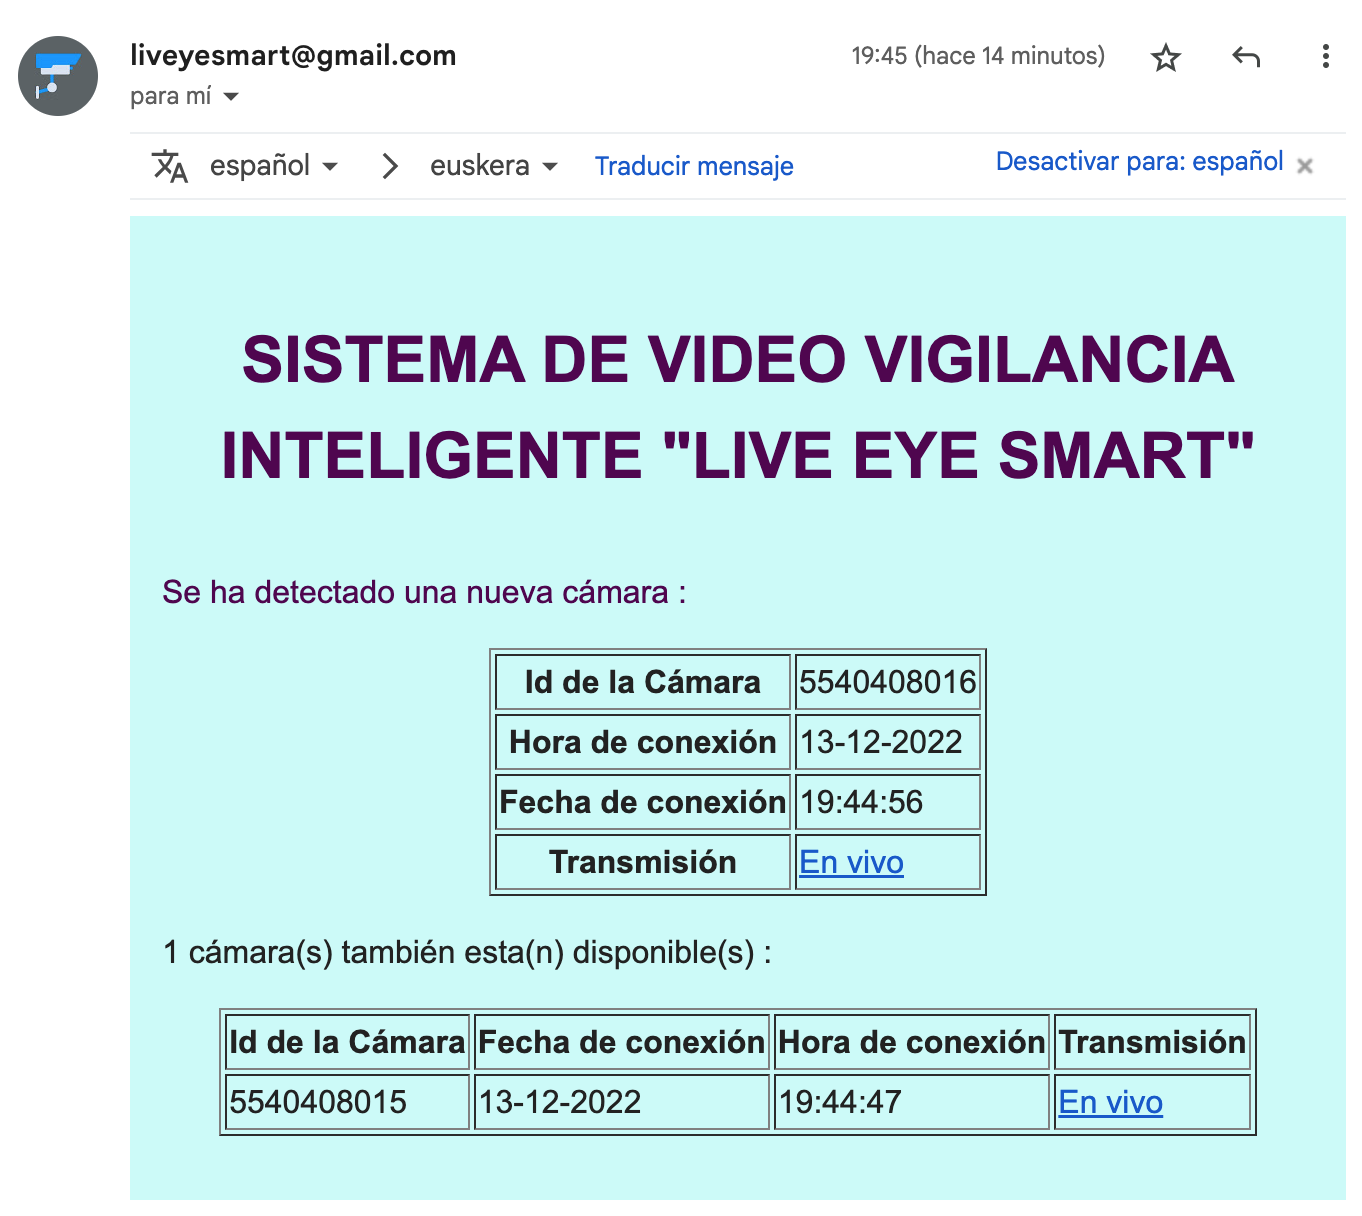
\includegraphics[width=10cm]{img/capitulo_6/mail2.png}
    \end{center}
    \begin{center}
        \caption{Notificación de más de una cámara conectada.}
        Fuente : Elaboración propia
        \label{notif_mail_n_cameras}
    \end{center}
\end{figure}

\section{Prueba de desconexión de cámaras}

En la tabla \ref{desconected_camera} se describe la prueba realizada en la desconexión de la única cámara conectada.

\begin{table}[H]
    \caption{Desconexión de una cámara conectada}
    \begin{center}
        \begin{tabular}{|>{\centering}p{0.3\textwidth}|m{0.6\textwidth}<{\centering}|} 
            \hline
            \textbf{Título de la prueba} & \textbf{Única cámara conectada y se desconecta} \\
            \hline
            \textbf{Descripción} & El servidor se encuentra en ejecución y la única instancia del módulo de cámaras se desconecta del servidor. No existen más cámaras conectadas.\\
            \hline
            \textbf{Comportamiento obtenido} & 
            \begin{itemize}
                \item El servidor registra la desconexión y lo muestra en consola.
                \item El servidor notifica al usuario por medio de correo electronico.
                \item La notificación provee información sobre la fecha y hora de la desconexión.
                \item La notificación detalla que no hay más conexiones.
            \end{itemize} \\ 
            \hline
            \textbf{Estado de prueba} & Exitoso \\
            \hline
        \end{tabular}
    \end{center}
    \begin{center}
        Fuente: Elaboración propia.
        \label{desconected_camera}
    \end{center}
\end{table}

En la figura \ref{desconected_camera_server} se muestra la interfaz del servidor sobre la desconexión de una cámara.

\begin{figure}[H]
    \begin{center}
        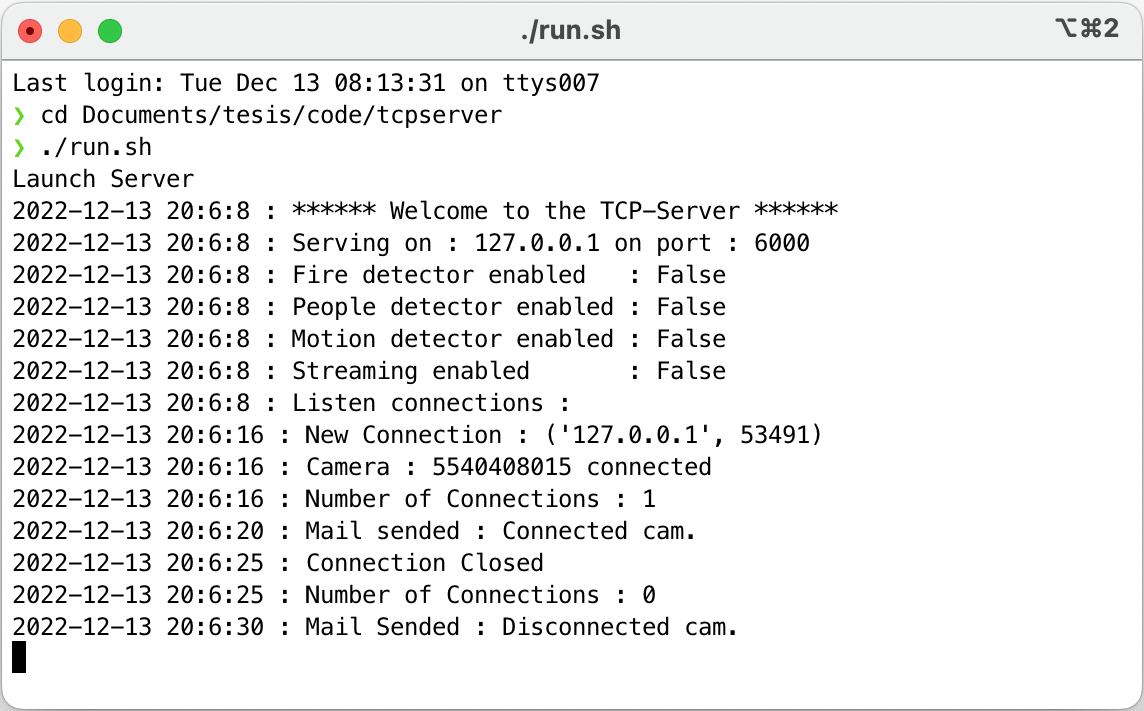
\includegraphics[width=12cm]{img/capitulo_6/cam_disconnected_1_cam.png}
    \end{center}
    \begin{center}
        \caption{Mensajes en consola del servidor - Única cámara desconectada.}
        Fuente: Elaboración propia
        \label{desconected_camera_server}
    \end{center}
\end{figure}

En la figura \ref{desconected_camera_server_mail} se visualiza el correo electrónico que es enviado al usuario después de la desconexión de una cámara.

\begin{figure}[H]
    \begin{center}
        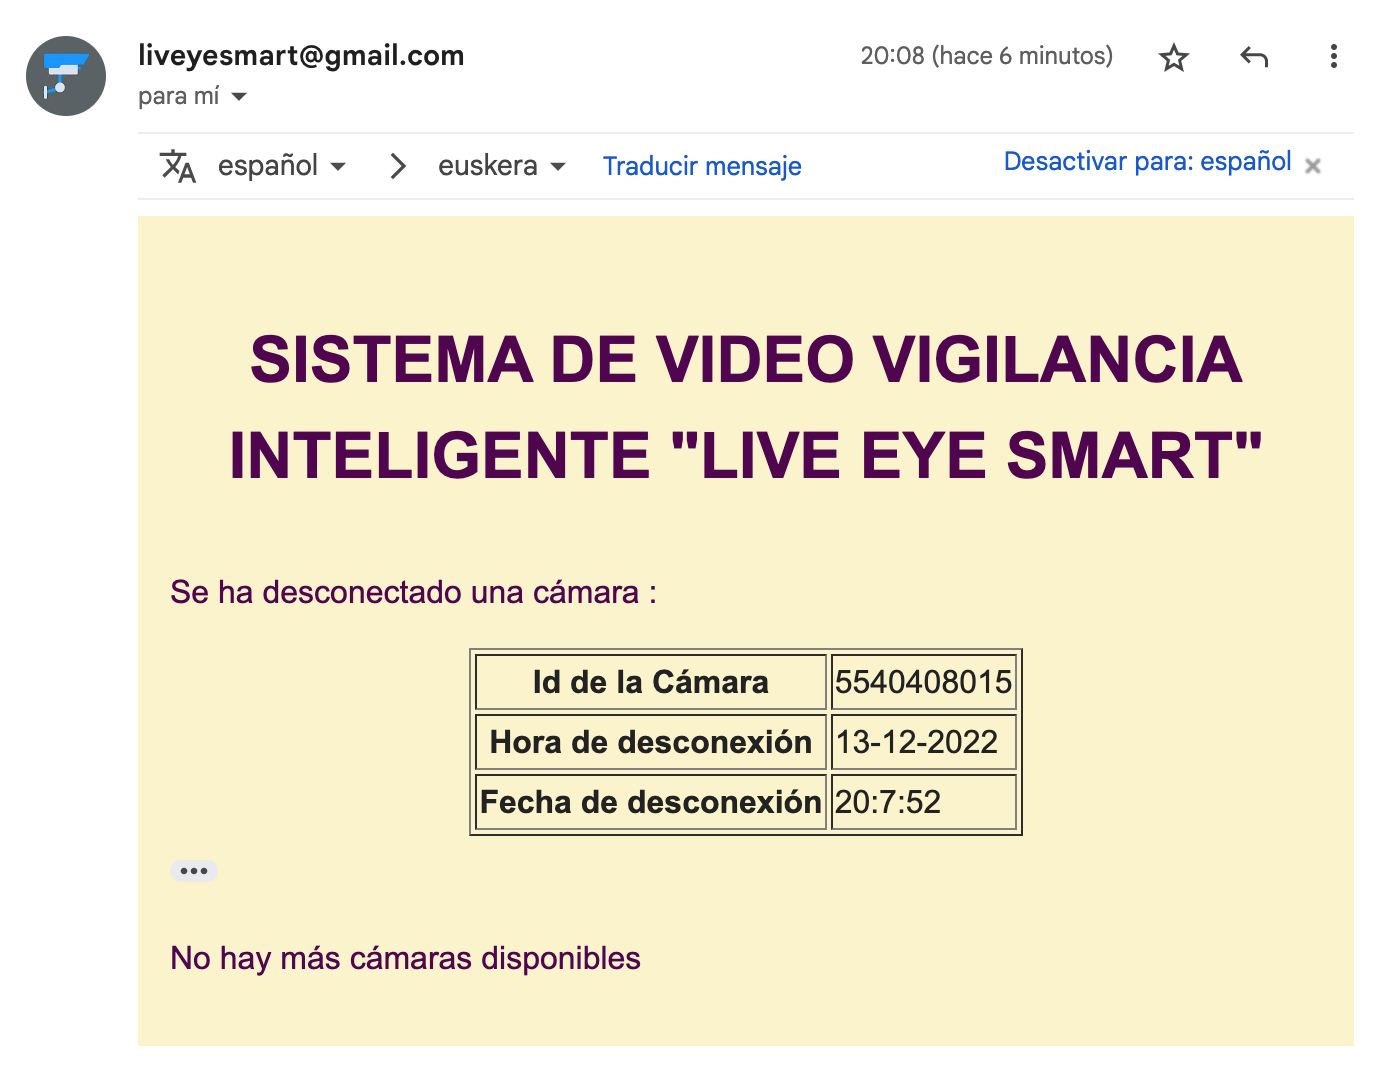
\includegraphics[width=12cm]{img/capitulo_6/mail4.png}
    \end{center}
    \begin{center}
        \caption{Notificación por correo - cámara desconectada.}
        Fuente: Elaboración propia
        \label{desconected_camera_server_mail}
    \end{center}
\end{figure}

En la tabla \ref{n_cameras_one_desconnected} se describe el proceso de desconexión de una de las cámaras conectadas:\\

\begin{table}[H]
    \caption{Desconexión de una de las cámaras}
    \begin{center}
        \begin{tabular}{|>{\centering}p{0.3\textwidth}|m{0.6\textwidth}<{\centering}|} 
            \hline
            \textbf{Título de la prueba} & \textbf{Una de las cámaras se desconecta} \\
            \hline
            \textbf{Descripción} & El servidor se encuentra en ejecución y una instancia del módulo de cámaras se desconecta del servidor. Existen más cámaras conectadas.\\
            \hline
            \textbf{Comportamiento obtenido} & 
            \begin{itemize}
                \item El servidor registra la desconexión y lo muestra en consola.
                \item El servidor notifica al usuario por medio de correo electrónico.
                \item La notificación provee información sobre la fecha y hora de la desconexión.
                \item La notificación detalla que no hay más conexiones.
                % \item El servidor acepta la conexión y lo muestra en consola.
                % \item El servidor notifica al usuario por medio de correo electronico.
                % \item La notificación provee información sobre la fecha y hora de la conexión, compartiendo el enlace para la transmisión en vivo.
            \end{itemize} \\ 
            \hline
            \textbf{Estado de prueba} & Exitoso \\
            \hline
        \end{tabular}
    \end{center}
    \begin{center}
        Fuente: Elaboración propia.
        \label{n_cameras_one_desconnected}
    \end{center}    
\end{table}

A continuación se muestra capturas del comportamiento esperado:

\begin{figure}[H]
    \begin{center}
        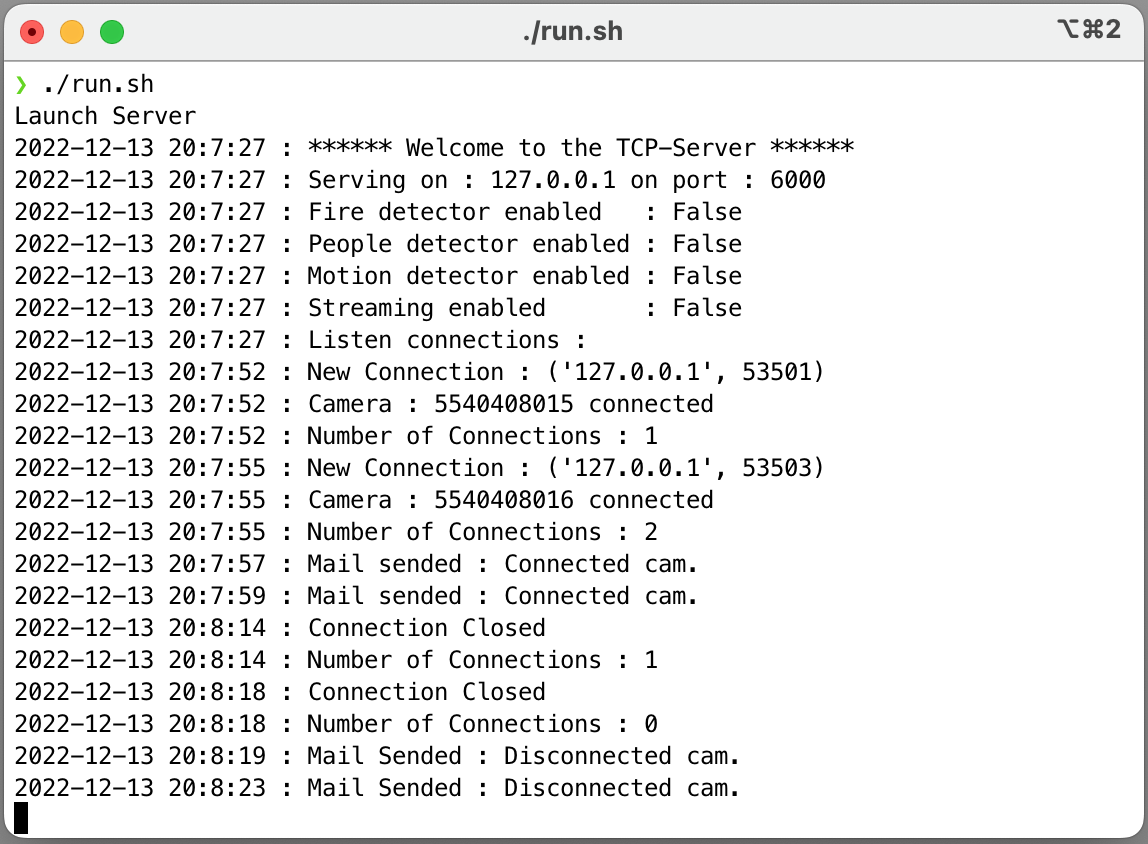
\includegraphics[width=12cm]{img/capitulo_6/cam_disconnected_n_cams.png}
    \end{center}
    \begin{center}
        \caption{Mensajes en consola del servidor - Cámara desconectada de varias.}
        Fuente : Elaboración propia
    \end{center}
\end{figure}

\begin{figure}[H]
    \begin{center}
        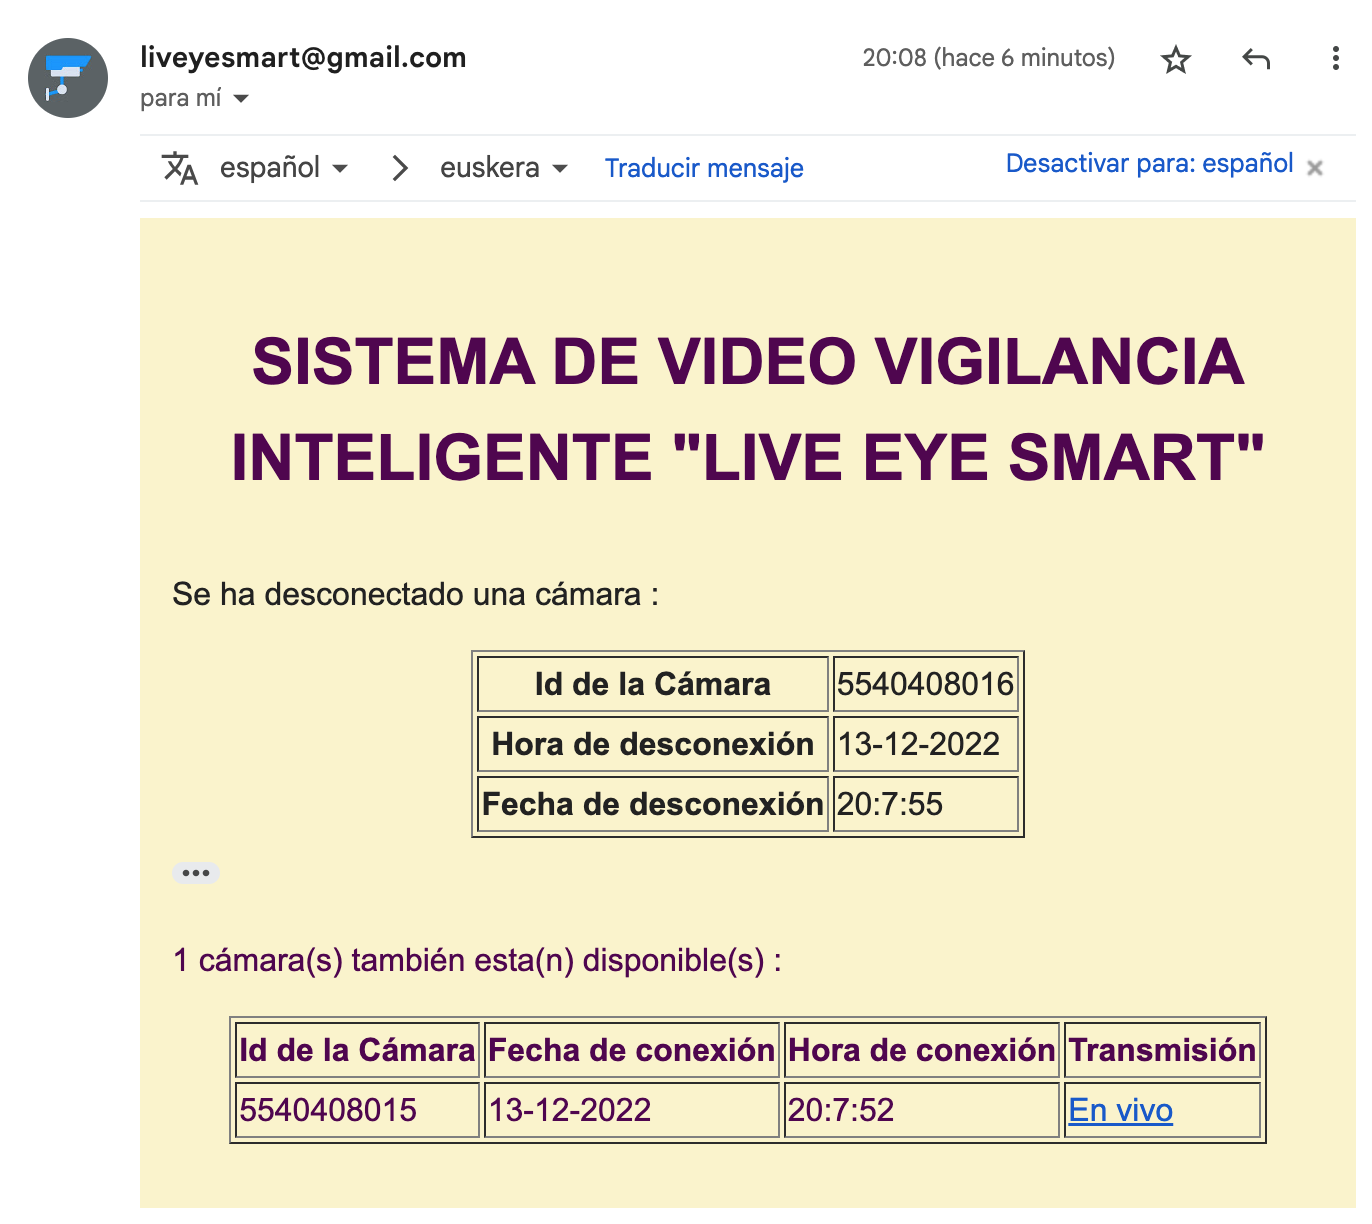
\includegraphics[width=10cm]{img/capitulo_6/mail3.png}
    \end{center}
    \begin{center}
        \caption{Notificación por correo - Cámara desconectada de varias.}
        Fuente : Elaboración propia
    \end{center}
\end{figure}

\section{Prueba de detección de fuego}

En la tabla \ref{table_fire_detection} se describe la prueba realizada sobre el detector de fuego.\\

\begin{table}[H]
    \caption{Detalle de prueba de detector de fuego}
    \begin{center}
        \begin{tabular}{|>{\centering}p{0.3\textwidth}|m{0.6\textwidth}<{\centering}|} 
            \hline
            \textbf{Título de la prueba} & \textbf{Detector de fuego identifica incidencia} \\
            \hline
            \textbf{Descripción} & El servidor se encuentra en ejecución y el proceso de identificación de fuego detecta una incidencia.\\
            \hline
            \textbf{Comportamiento obtenido} & 
            \begin{itemize}
                \item El servidor captura los fotogramas como prueba de la incidencia.
                \item El servidor notifica al usuario por medio de correo electronico.
                \item La notificación provee información sobre la fecha y hora de la incidencia, compartiendo el enlace para la transmisión en vivo.
            \end{itemize} \\ 
            \hline
            \textbf{Estado de prueba} & Exitoso \\
            \hline
        \end{tabular}
    \end{center}
    \begin{center}
        Fuente: Elaboración propia.
        \label{table_fire_detection}
    \end{center}
\end{table}

En la figura \ref{camera_fire_detector} se visualiza el módulo de cámaras durante la detección.

\begin{figure}[H]
    \begin{center}
        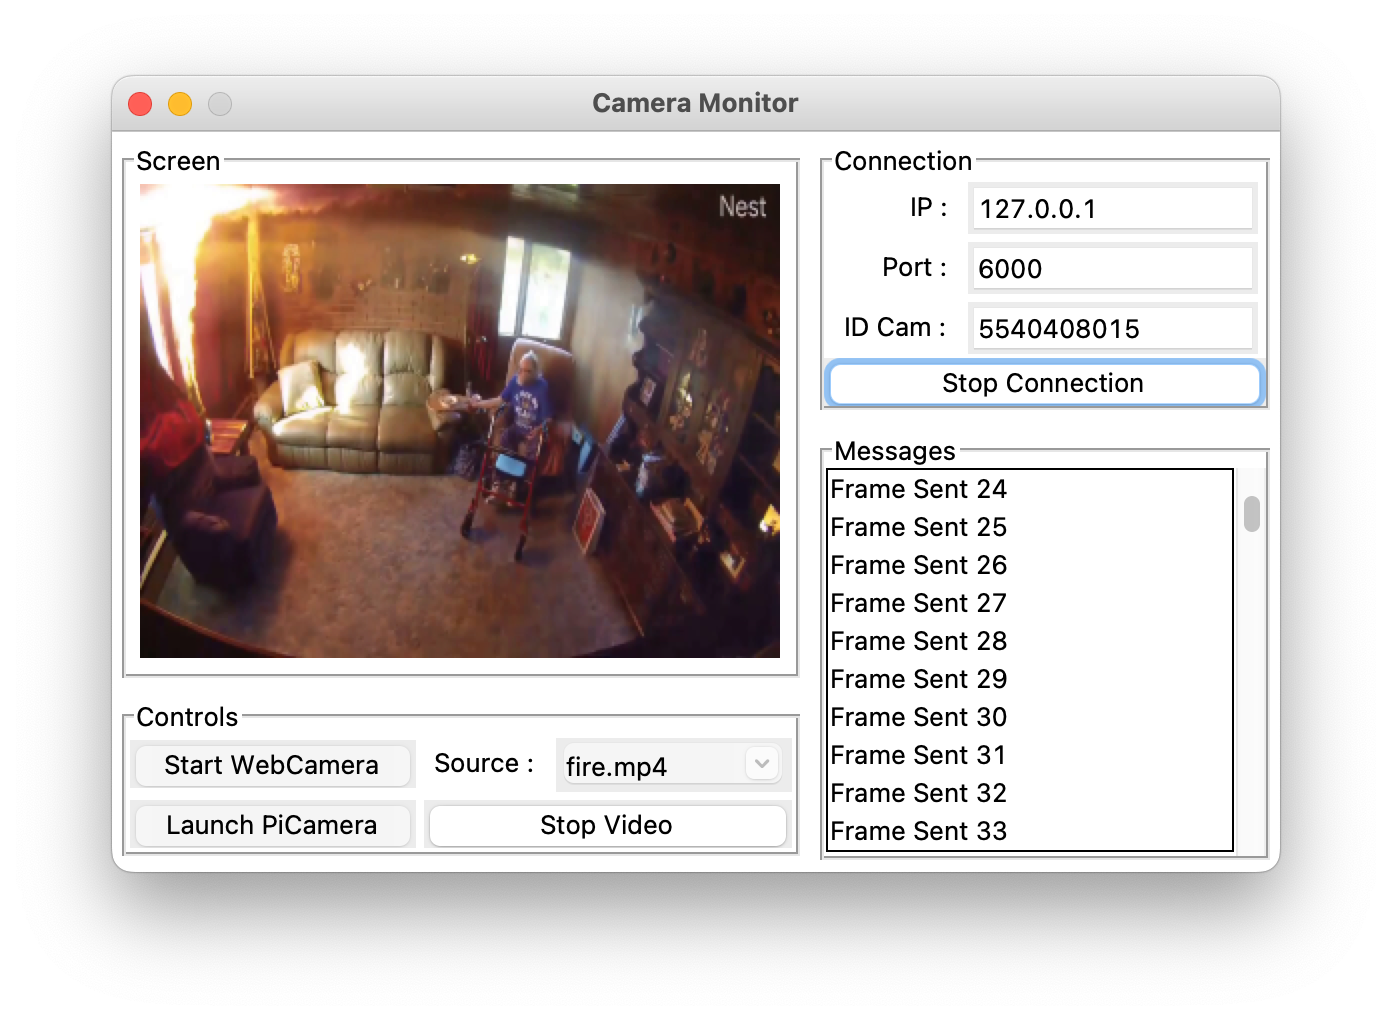
\includegraphics[width=11cm]{img/capitulo_6/fire.png}
    \end{center}
    \begin{center}
        \caption{Presencia de fuego en la escena.}
        Fuente : Elaboración propia
        \label{camera_fire_detector}
    \end{center}
\end{figure}

En la figura \ref{mail_fire_detection} se visualiza la notificación por correo electrónico despues de la detección.

\begin{figure}[H]
    \begin{center}
        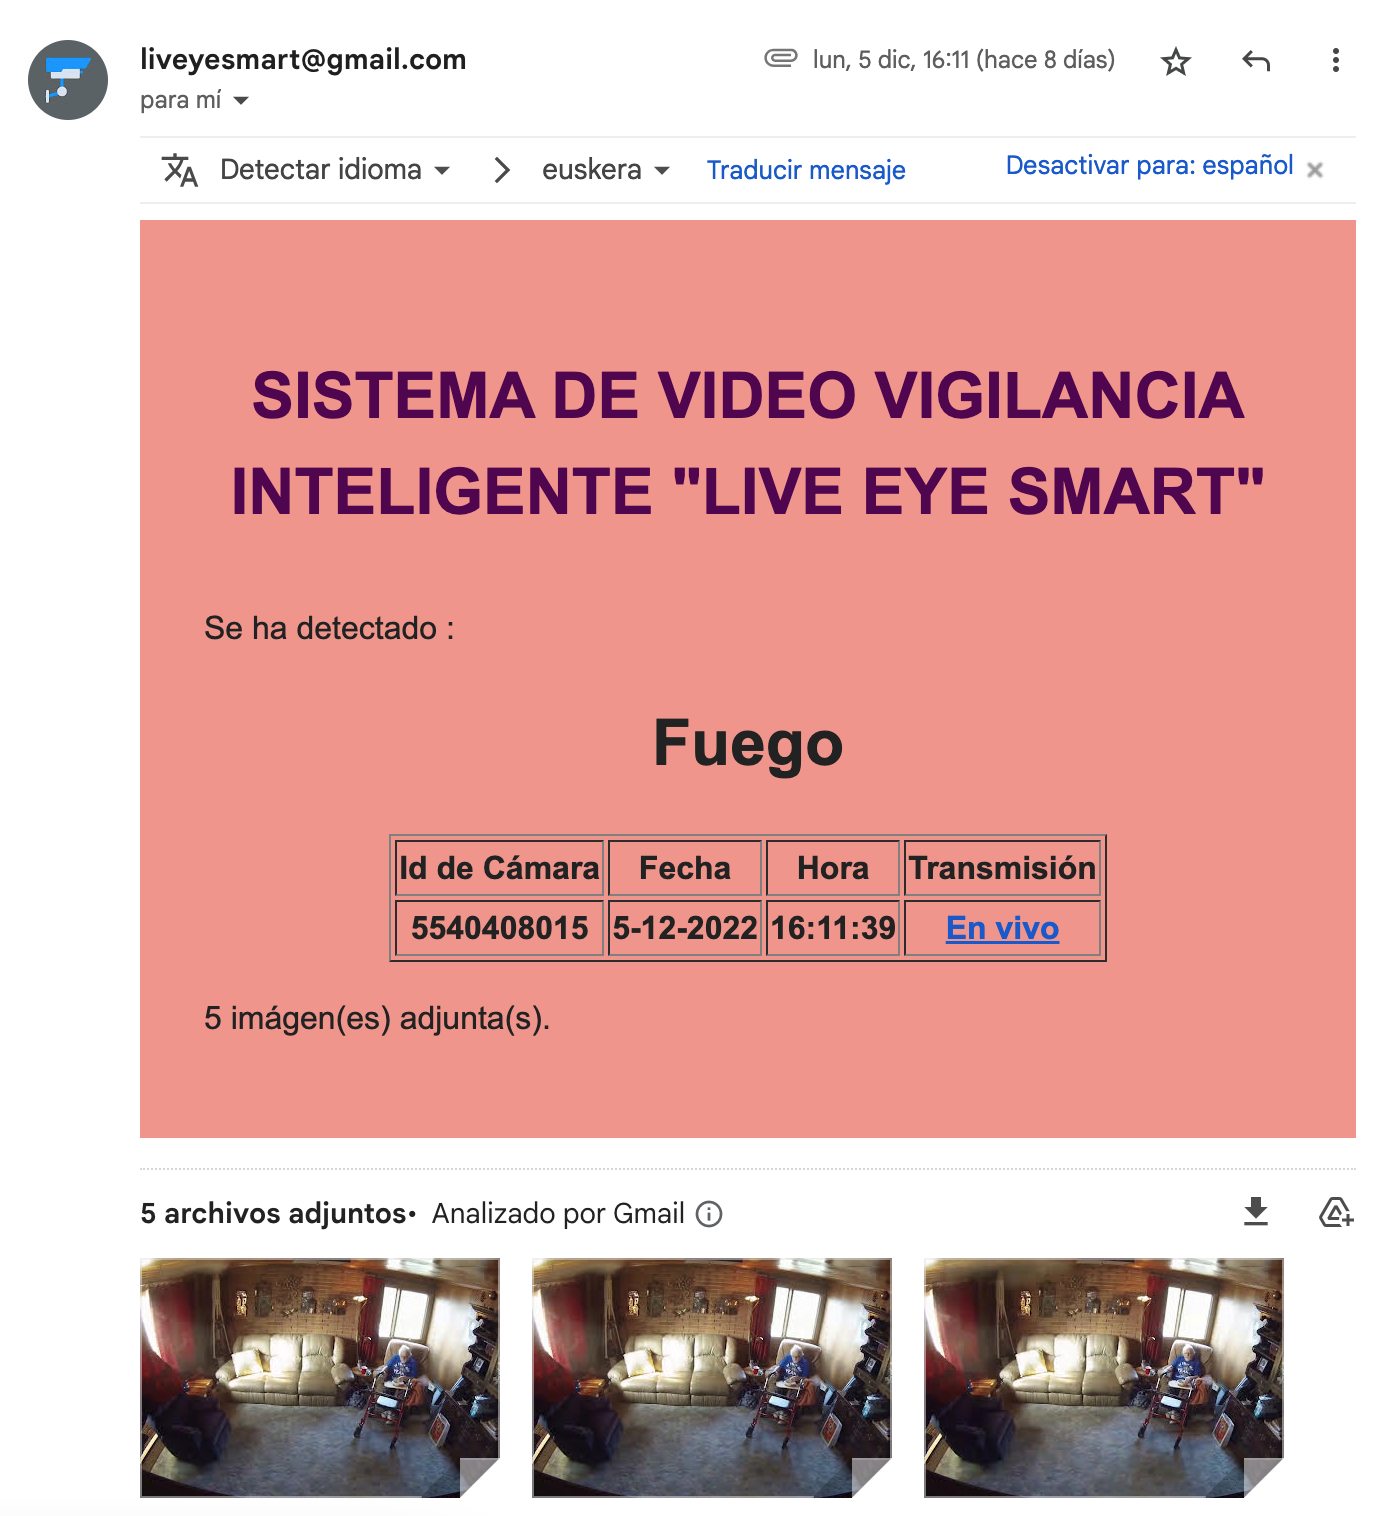
\includegraphics[width=9cm]{img/capitulo_6/mail_fire.png}
    \end{center}
    \begin{center}
        \caption{Notificación por correo electrónico - Alerta de fuego.}
        Fuente : Elaboración propia
        \label{mail_fire_detection}
    \end{center}
\end{figure}

\section{Prueba de detección de silueta humana}

En la tabla \ref{table_human_siluete} se describe la prueba realizada para la detección de intrusos.

\begin{table}[H]
    \caption{Detalle de prueba de detector de silueta humana}
    \begin{center}
        \begin{tabular}{|>{\centering}p{0.3\textwidth}|m{0.6\textwidth}<{\centering}|} 
            \hline
            \textbf{Título de la prueba} & \textbf{Detector de silueta humana identifica incidencia} \\
            \hline
            \textbf{Descripción} & El servidor se encuentra en ejecución y el proceso de identificación de silueta humana detecta una incidencia.\\
            \hline
            \textbf{Comportamiento obtenido} & 
            \begin{itemize}
                \item El servidor captura los fotogramas como prueba de la incidencia.
                \item El servidor notifica al usuario por medio de correo electronico.
                \item La notificación provee información sobre la fecha y hora de la incidencia, compartiendo el enlace para la transmisión en vivo.
            \end{itemize} \\ 
            \hline
            \textbf{Estado de prueba} & Exitoso \\
            \hline
        \end{tabular}
    \end{center}
    \begin{center}
        Fuente: Elaboración propia.
        \label{table_human_siluete}
    \end{center}
\end{table}

En la figura \ref{camera_human_siluete} se visualiza el funcionameinto del módulo de cámaras durante la prueba.

\begin{figure}[H]
    \begin{center}
        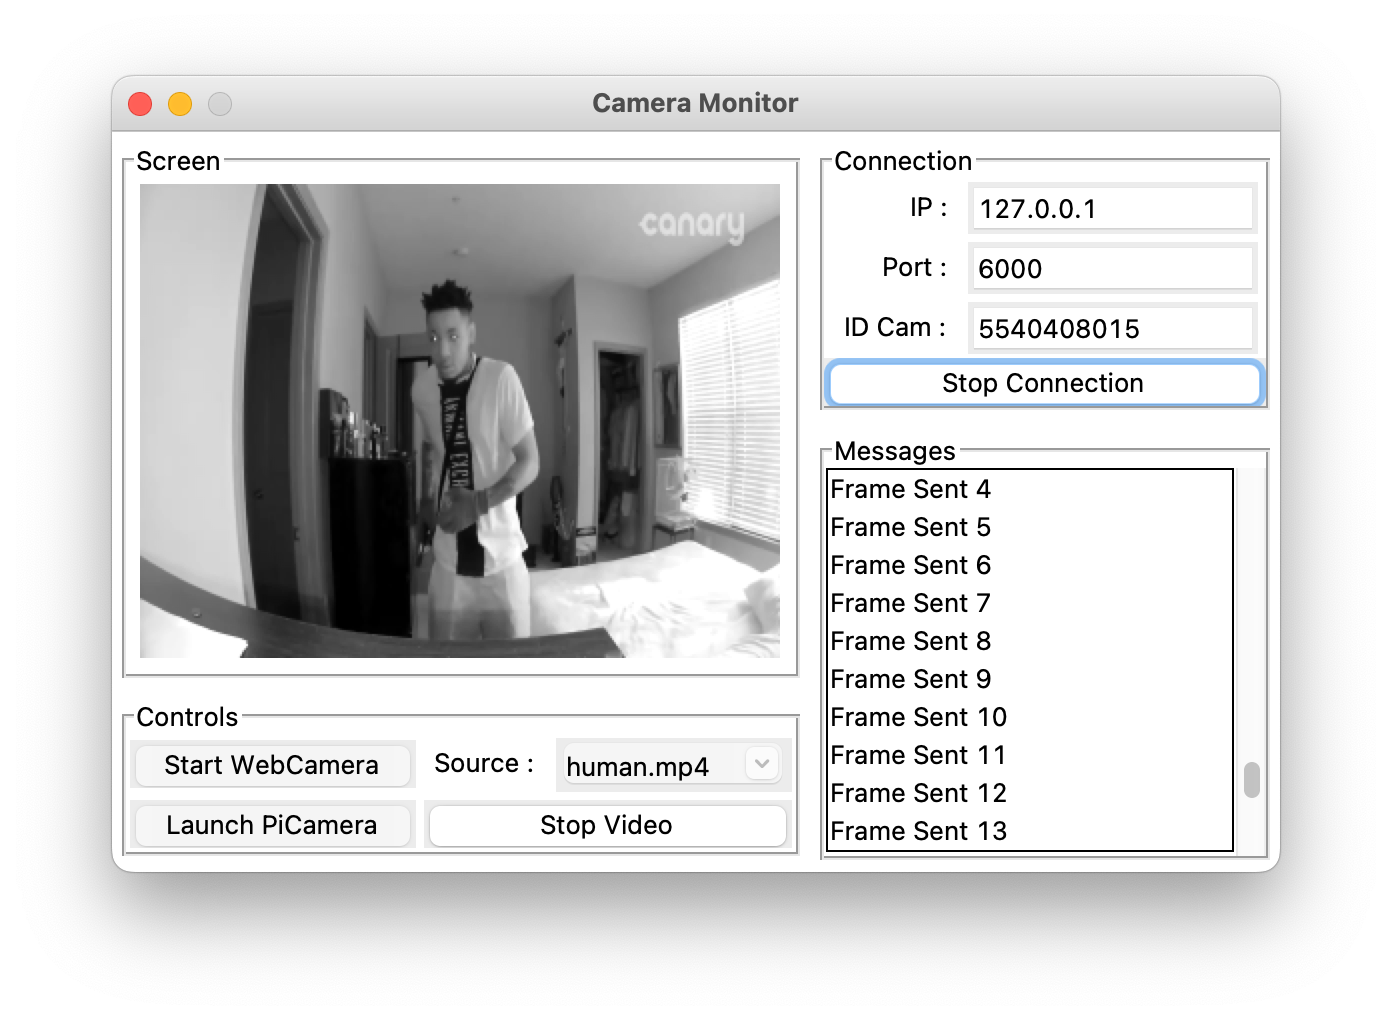
\includegraphics[width=12cm]{img/capitulo_6/human.png}
    \end{center}
    \begin{center}
        \caption{Visualización en módulo de cámaras - Presencia de intruso en la escena.}
        Fuente : Elaboración propia
        \label{camera_human_siluete}
    \end{center}
\end{figure}

En la figura \ref{mail_human_siluete} se visualiza el correo electrónico como notificación enviado al usuario después de la detección de intrusos.

\begin{figure}[H]
    \begin{center}
        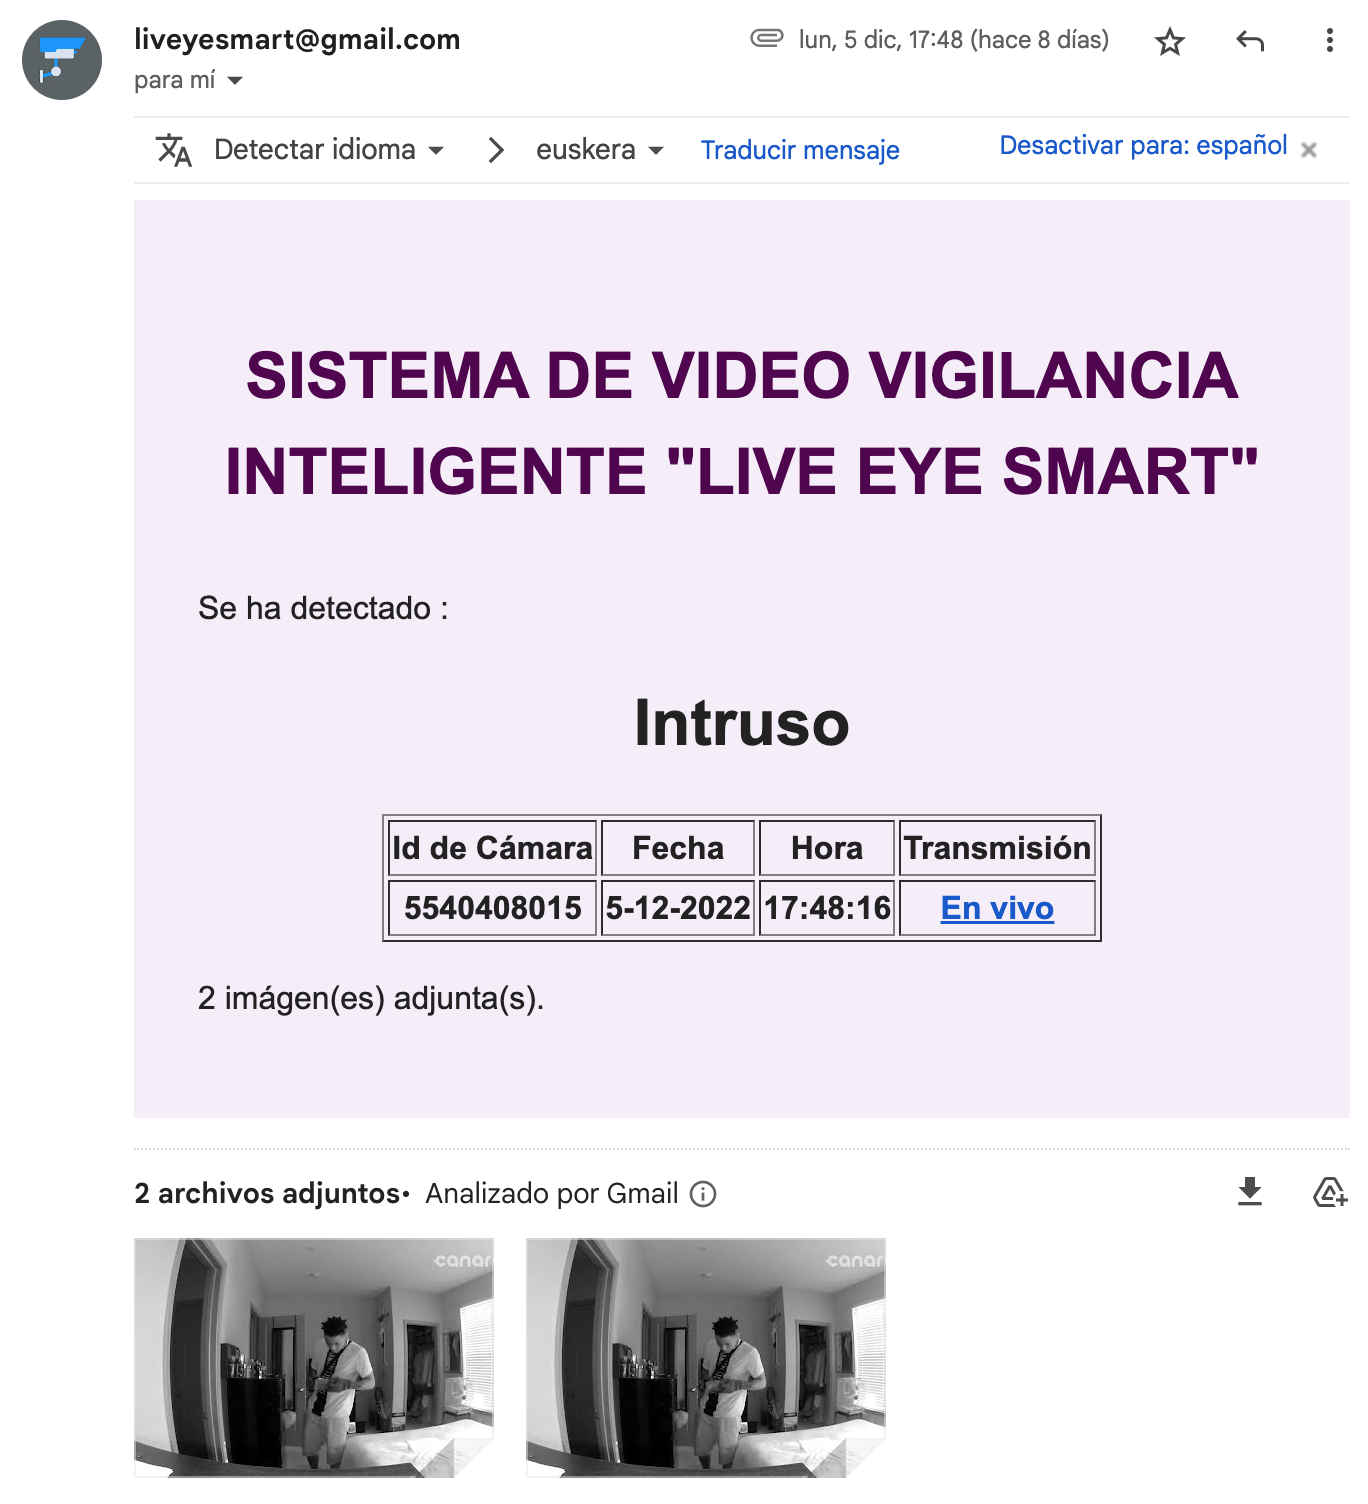
\includegraphics[width=8cm]{img/capitulo_6/mail_human.png}
    \end{center}
    \begin{center}
        \caption{Correo electrónico para alerta de intrusos.}
        Fuente : Elaboración propia
        \label{mail_human_siluete}
    \end{center}
\end{figure}

\section{Prueba de detección de movimiento}

En la tabla \ref{table_movement_detection} se detalla la prueba realizada sobre el detector de movimiento.\\

\begin{table}[H]
    \caption{Detalle de prueba de detector de movimiento}
    \begin{center}
        \begin{tabular}{|>{\centering}p{0.3\textwidth}|m{0.6\textwidth}<{\centering}|} 
            \hline
            \textbf{Título de la prueba} & \textbf{Detector de movimiento identifica incidencia} \\
            \hline
            \textbf{Descripción} & El servidor se encuentra en ejecución y el proceso de identificación de movimiento detecta una incidencia.\\
            \hline
            \textbf{Comportamiento obtenido} & 
            \begin{itemize}
                \item El servidor captura los fotogramas como prueba de la incidencia.
                \item El servidor notifica al usuario por medio de correo electronico.
                \item La notificación provee información sobre la fecha y hora de la incidencia, compartiendo el enlace para la transmisión en vivo.
            \end{itemize} \\ 
            \hline
            \textbf{Estado de prueba} & Exitoso \\
            \hline
        \end{tabular}
    \end{center}
    \begin{center}
        Fuente: Elaboración propia.
        \label{table_movement_detection}
    \end{center}
\end{table}

En la figura \ref{camera_movement} se visualiza el comportamiento de la cámara durante la prueba.

\begin{figure}[H]
    \begin{center}
        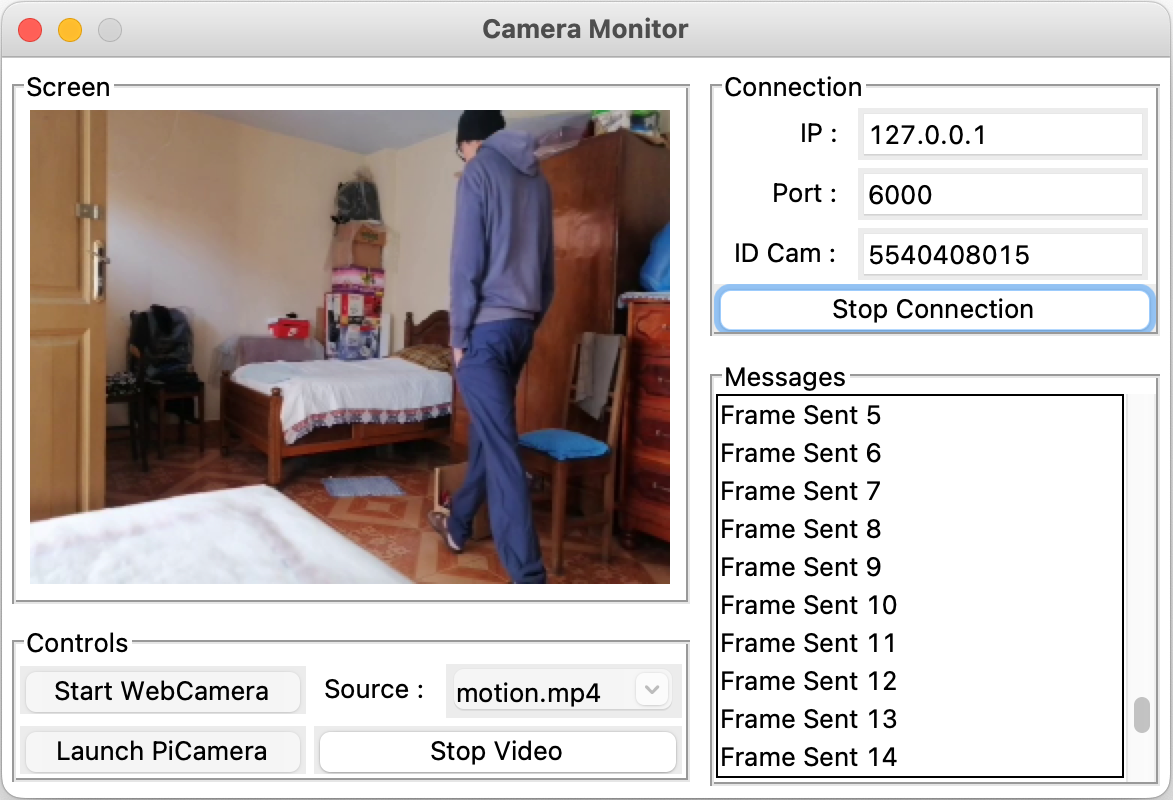
\includegraphics[width=10cm]{img/capitulo_6/motion.png}
    \end{center}
    \begin{center}
        \caption{Visualización en módulo de cámaras - Movimiento.}
        Fuente : Elaboración propia
        \label{camera_movement}
    \end{center}
\end{figure}

En la figura \ref{mail_movement} se visualiza el correo electrónico que se envia al usuario como notificación con capturas adjuntas sobre la detección.

\begin{figure}[H]
    \begin{center}
        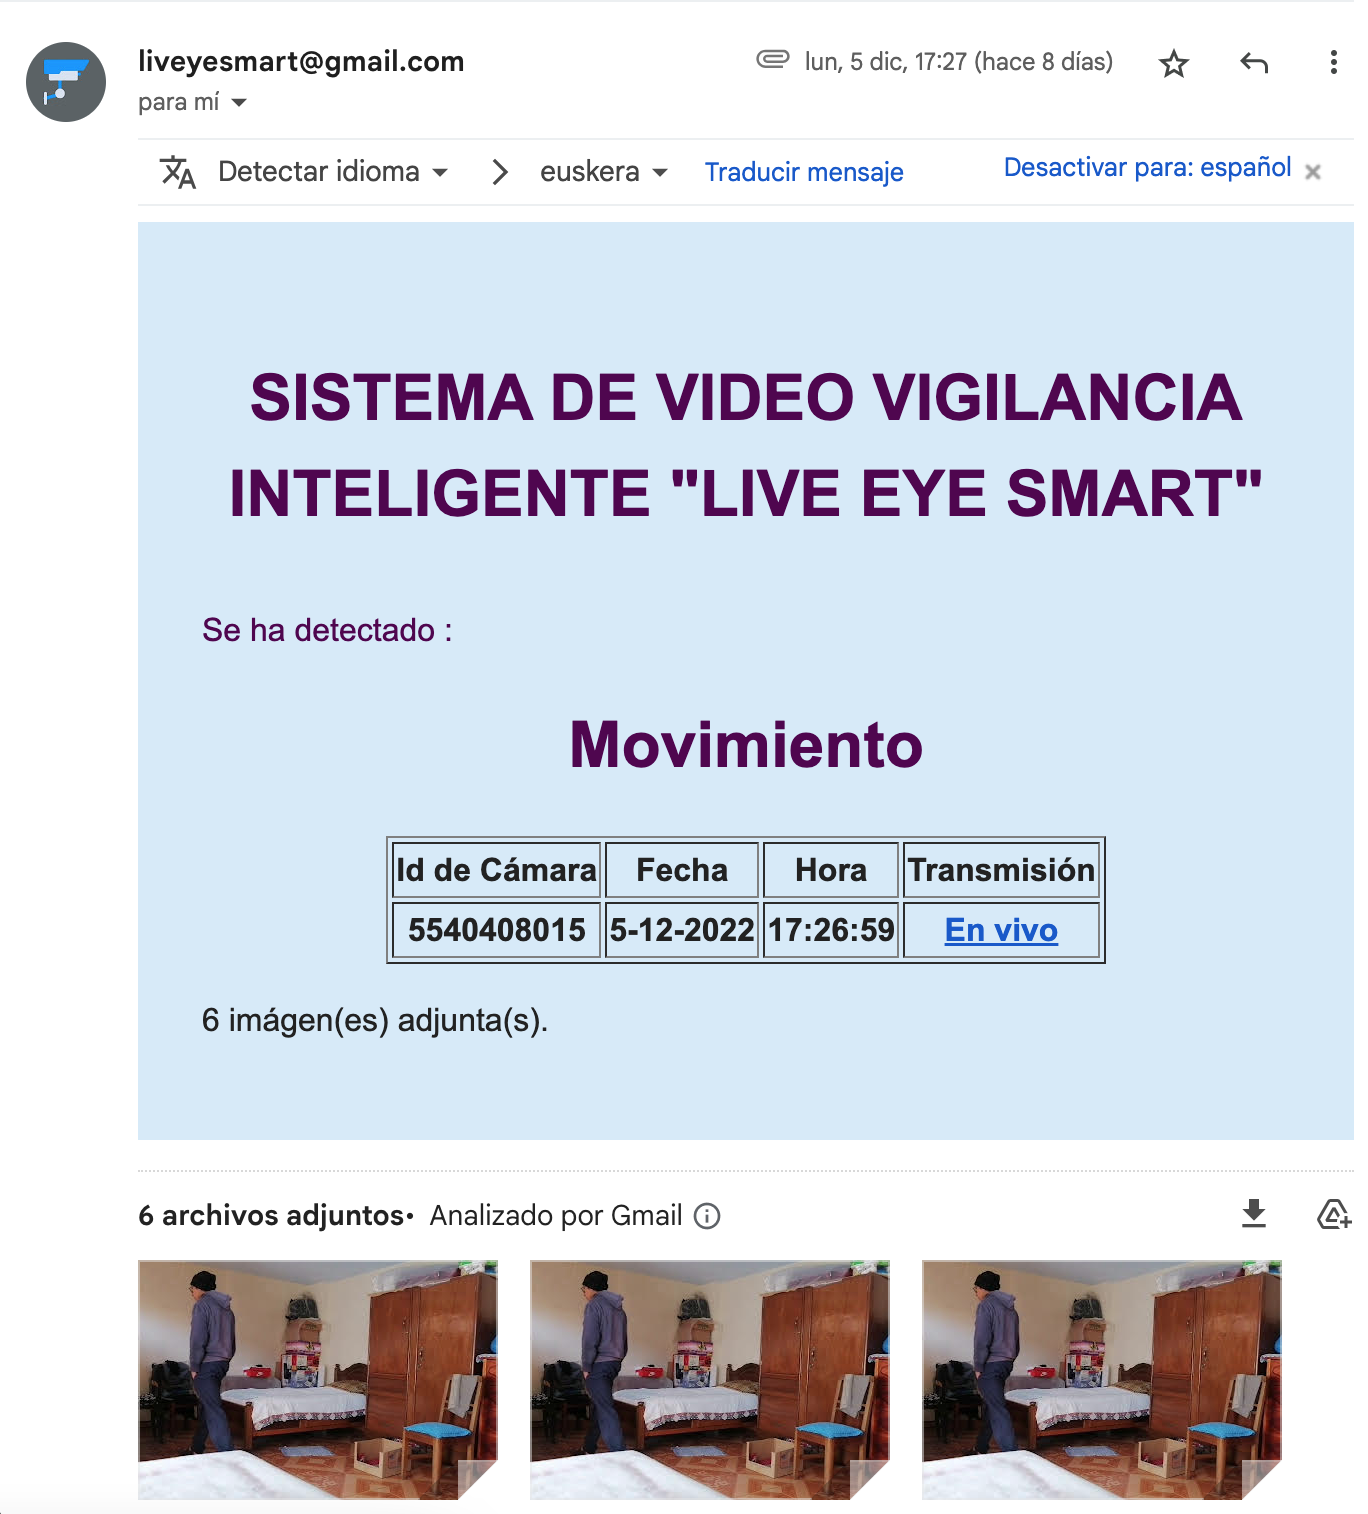
\includegraphics[width=9cm]{img/capitulo_6/mail_motion.png}
    \end{center}
    \begin{center}
        \caption{Detalle de notificación por correo electrónico - Alerta de movimiento.}
        Fuente : Elaboración propia
        \label{mail_movement}
    \end{center}
\end{figure}

\section{Prueba de transmisión de video en vivo}

En la tabla \ref{stream_camera} se describe la prueba de la transmisión en vivo.\\

\begin{table}[H]
    \caption{Detalle de prueba de la transmisión de video en vivo.}
    \begin{center}
        \begin{tabular}{|>{\centering}p{0.3\textwidth}|m{0.6\textwidth}<{\centering}|} 
            \hline
            \textbf{Título de la prueba} & Transmisión de video\\
            \hline
            \textbf{Descripción} & El servidor se encuentra en ejecución. El usuario ingresa al enlace adjunto en la notificación de conexión para la transmisión de video en vivo.\\
            \hline
            \textbf{Comportamiento obtenido} & 
            \begin{itemize}
                \item El servidor registra la conexión y se muestra en consola.
                \item El servidor comienza con la decodificación video.
                \item La notificación provee información del enlace para su transmisión en vivo.
                \item La transmisión se visualiza en un reproductor de video adaptativo en el navegador.
            \end{itemize} \\ 
            \hline
            \textbf{Estado de prueba} & Exitoso \\
            \hline
        \end{tabular}
    \end{center}
    \begin{center}
        Fuente: Elaboración propia.
        \label{stream_camera}
    \end{center}
\end{table}

En la figura \ref{mod_camera_stream} se visualiza el estado del módulo de cámara durante la transmisión:\\

\begin{figure}[H]
    \begin{center}
        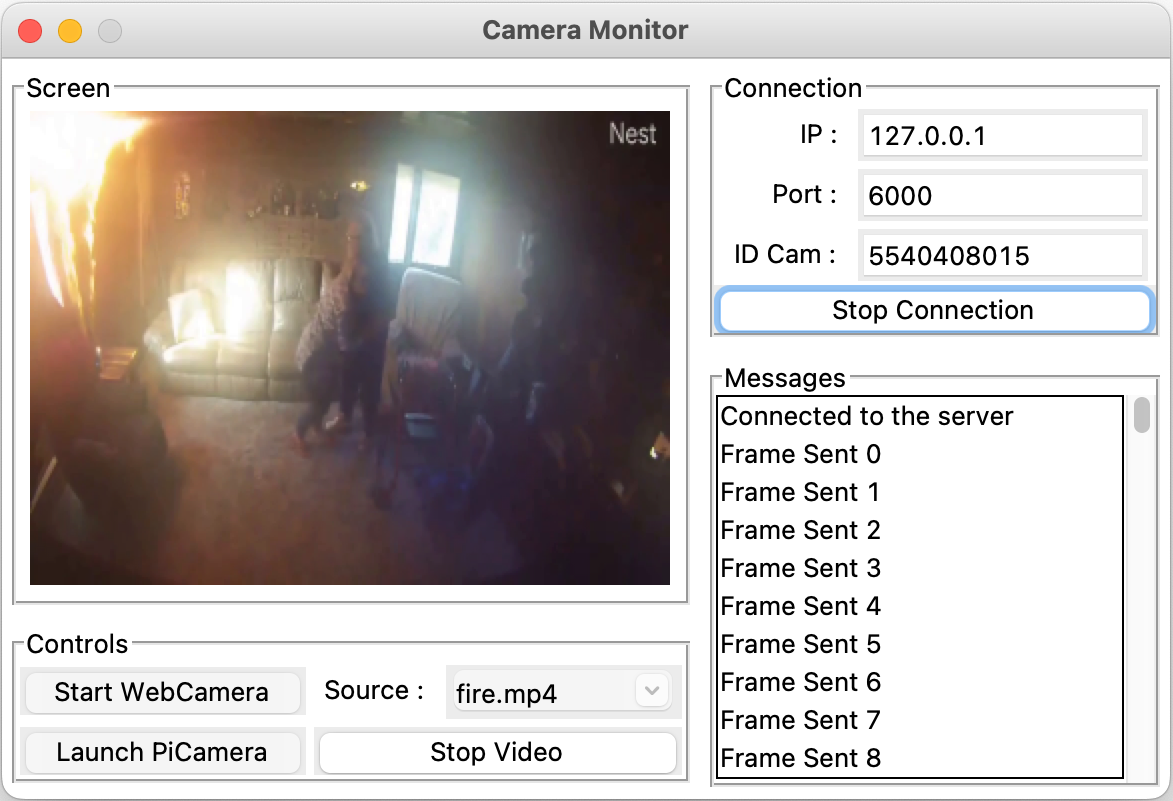
\includegraphics[width=11cm]{img/capitulo_6/stream.png}
    \end{center}
    \begin{center}
        \caption{Visualización en módulo de cámaras.}
        Fuente : Elaboración propia
        \label{mod_camera_stream}
    \end{center}
\end{figure}

En la figura \ref{stream_chrome} se visualiza la transmisión de video en vivo por medio de un reproductor de video adaptativo directamente en un navegador web.

\begin{figure}[H]
    \begin{center}
        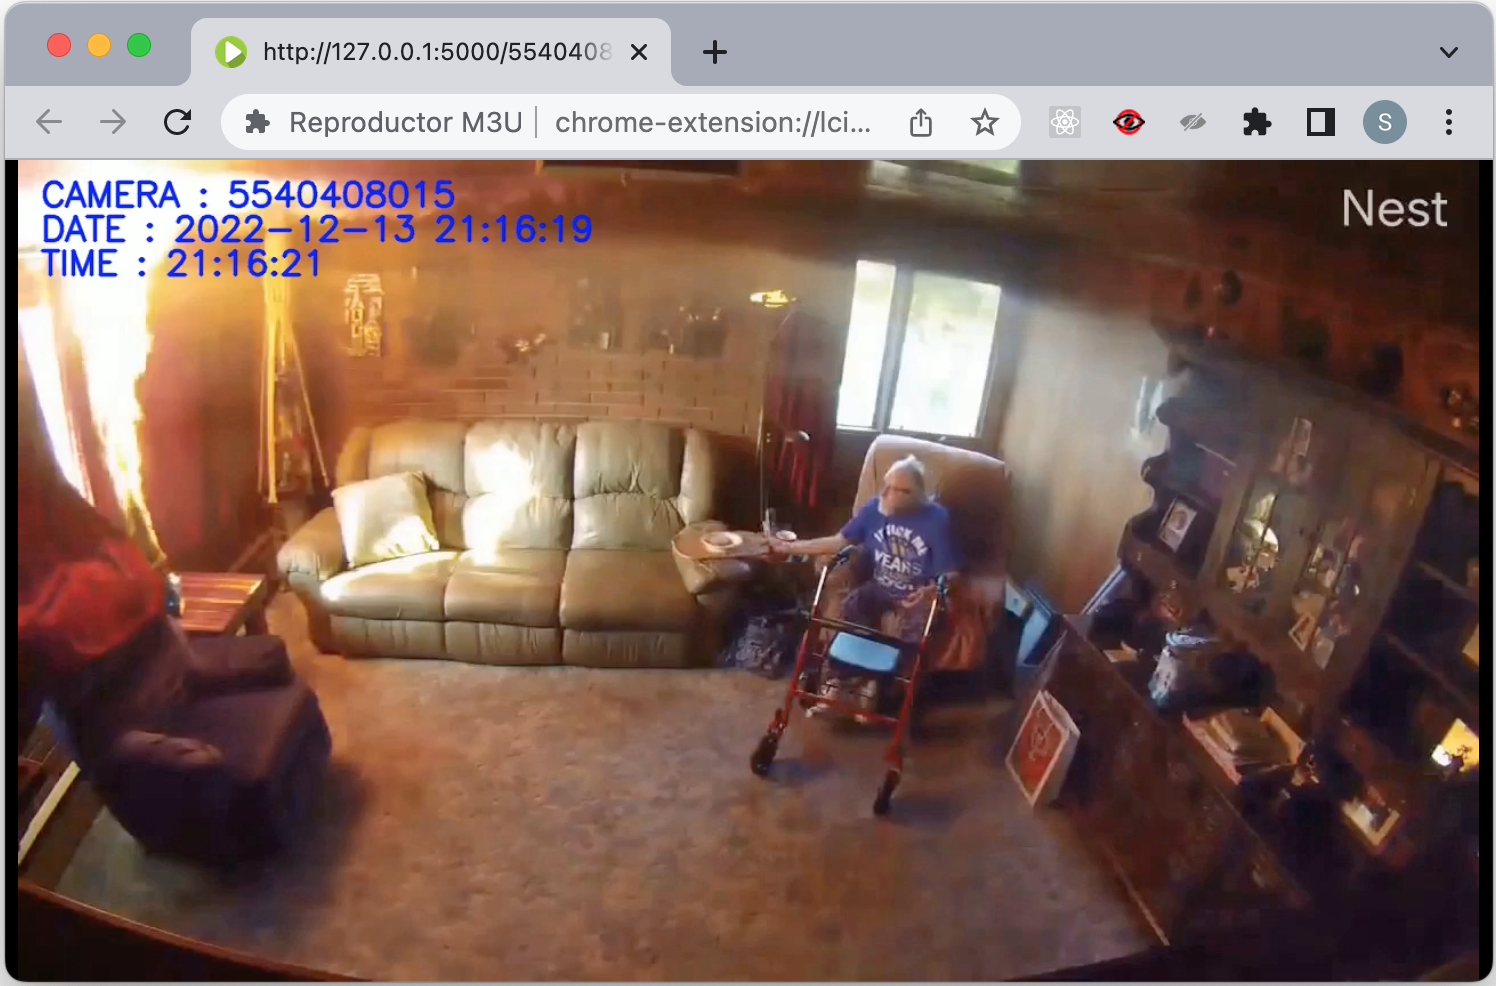
\includegraphics[width=15cm]{img/capitulo_6/stream_web.png}
    \end{center}
    \begin{center}
        \caption{Reproductor web de video en Streaming.}
        Fuente : Elaboración propia
        \label{stream_chrome}
    \end{center}
\end{figure}

Las pruebas re acpetación realizadas sobre el sistema de video-vigilancia intelignete implementado prueban: la conexón y desconexión de cámaras al sistema, como también las notificaciones según a lo que llegue a identificarse.

% \begin{itemize}
%     \item Prueba de conexión de cámaras.
%     \item Prueba de desconexión de cámaras.
%     \item Prueba de detección de fuego y notificación.
%     \item Prueba de detección de silueta humana y notificación.
%     \item Prueba de detección de movimiento y notificación.
%     \item Prueba de transmisión de video en vivo.
% \end{itemize}
